\section{Обучение с подкреплением} \label{ch1:rl}

Хотя алгоритмы \hyperref[acr:rl]{RL} эффективно решают различные задачи, им не хватает масштабируемости и размерности.

С ростом глубоких нейронных сетей в последние годы обучение с подкреплением начинает использовать их функции приближения и представления свойств \cite{HORNIK1991251}. Это помогает преодолеть недостатки алгоритмов обучения с подкреплением.

Это устраняет необходимость описывать свойства вручную, позволяя обучать модели, способные непосредственно выводить оптимальные действия, на основе необработанного и высокоразмерного ввода с сенсоров. Это проиллюстрировано на \firef{fig:DRL-flow}.

\begin{figure}[ht!]
    \center
    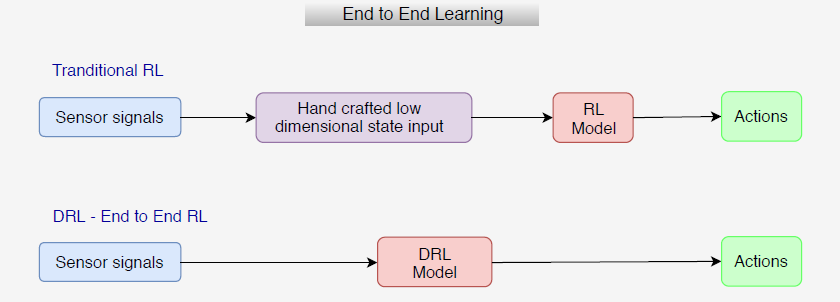
\includegraphics [scale=0.65] {my_folder/images/ch1/DRL-flow.png}
    \caption{Cравнение DRL и традиционной RL, где необходимо явно указать, какие действия производить в каких состояниях. Использование глубокой нейронной сети в DRL позволяет обучаться и принимать решения на основе необработанного сенсорного ввода}
    \label{fig:DRL-flow}
\end{figure}

Таким образом, использование ИНС в обучении с подкреплением создаёт новую область – глубокое обучение с подкреплением (Deep Reinforcement Learning, DRL).

\subsection{Алгоритмы глубокого обучения с подкреплением}

Два основных подхода к обучению с подкреплением: основанные на value-функции и на градиенте политики. $Q$-обучение~--- вероятностный value итерационный метод, цель которого~--- оценка $Q$-функции. Методы градиента политики же стараются оптимизировать политику напрямую.

Здесь нужно рассказать о \hyperref[acr:mdp]{марковском процессе принятия решений} (Markov Decision Process, MDP).

\subsubsection{Марковский процесс принятия решений}

Свойство Маркова означает, что следующее состояние зависит только от текущего состояния, тем самым, при принятии решения, можно игнорировать все прошлые состояния и учитывать только текущее.

Процесс обучения с подкреплением является формой \hyperref[acr:mdp]{МППР}. Он состоит из нескольких элементов:

\begin{itemize}
    \item набор состояний окружающей среды $S$;
    \item набор действий $A$;
    \item динамика перехода $T(s_{(t+1)}|s_t, a_t)$, которая описывает распределение новых состояний $s_{t+1}$, в которые может попасть агент, совершив действие $a_t$ в состоянии $s_t$;
    \item функция награды $R(s_t; a_t; s_{t+1})$;
    \item дискаунт фактор $\gamma \in [0, 1]$ для экспоненциального снижения будущих наград.
\end{itemize}

Политика $\pi$ сопоставляет состояниям распределение вероятностей принятия действий: ${\pi : S \to p(A = a|S)}$.

Эпизод~--- это предопределённый период времени, когда среда, начиная со случайного состояния, порождает серию переходов. Переходы в эпизоде можно рассматривать как траекторию политики.

Сумма наград, собранных в траектории политики: ${R = \sum_{t=0}^{T-1} \gamma^t r_{t+1}}$.

Цель обучения с подкреплением состоит в том, чтобы получить оптимальную политику ${\pi^*}$, которая максимизирует ожидаемую награду из всех состояний: ${\pi^* = argmax_x \mathbb{E} [R|\pi]}$ \cite{Otterlo2012ReinforcementLA}.

\subsection{Подход, основанный на функции состояния (Value Based подход)}

Этот подход состоит в том, чтобы оптимизировать значение функции $V(s)$.

Value-функция~--— это функция, которая сообщает нам максимальное ожидаемое будущее вознаграждение, которое агент получит в каждом состоянии. Значение каждого состояния — это общая сумма вознаграждений, на которую агент может рассчитывать в будущем, начиная с этого состояния.

\subsubsection{$Q$-обучение}

Функция состояния-значения (state-value function) $V^\pi (s) = \mathbb{E}[R|s, \pi]$~--- ожидаемая награда с данными состоянием $s$ и политикой $\pi$. В то же время в RL такой переход $T$ не всегда возможен, поэтому обычно используется другая функция состояния-значения или функция качества ${Q^\pi(s,a) = \mathbb{E}[R|s, a, \pi]}$. Оптимальная политика получается через выбор на каждом шаге действия, которое максимизирует $Q$-функцию \cite{SuttonAndBarto-RL-Introduction-p107}. $Q$-обучение~--- это алгоритм без политики (off-policy), так как он жадно выбирает действие исходя из текущего состояния, вместо того, чтобы следовать политике.

Для рекурсивного вычисления $Q^\pi$ применяется уравнение Беллмана:

\begin{equation}
    \label{eq:q-learning-bellmanEq}
    Q^\pi(s_t, a_t) = \mathbb{E}_{s_{t+1}}[r_{t+1} + \gamma Q^\pi (s_{t+1}, \pi(s_{t+1}))].
\end{equation}

Традиционное $Q$-обучение способно сформулировать оптимальную политику обучением состояние-действие-значение функции. Однако, оно предназначено для дискретных пространств действий с малым количеством измерений и не способно решать более-менее сложные задачи.

\subsubsection{Глубокая $Q$-сеть (DQN)}

Глубокая $Q$-сеть (DQN)~--- вариант $Q$-обучения, который использует глубокую сверточную нейронную сеть для вычисления $Q$-функции. Является прорывом в обучении с подкреплением. \cite{bertsekas1996neuro}

DQN была применена в игре Atari и достигла производительности, сопоставимой с человеческим уровнем. \cite{Mnih2015}

Для решения проблемы нестабильности и расхождения нелинейных функций аппроксиматоров, таких как нейронные сети, был применён метод Experience Replay \cite{Lin1992ReinforcementLF}. Идея Experience Replay состоит в том, чтобы равномерно рандомизировать предыдущие переходы при обучении модели, что нарушает корреляцию последовательности наблюдений. Опыт агента ${e_t = (s_t, a_t, r_t, s_{t+1)}}$ на каждом шаге $t$ сохраняется в буфер ${D_t = ({e_1, ..., e_t})}$. Во время тренировки модели случайным образом извлекается небольшая часть опыта ${(s; a; r; s') \sim U(D)}$.

Еще одно новое приложение в DQN заключается в том, что создаются две $Q$-сети.
Текущая $Q$-сеть $Q(s, a; \theta_i)$ обновляется итеративно во время обучения, а целевая $Q$-сеть $Q(s', a'; \theta_i)$ используется для получения целевого $Q$-значения и обновляется только периодически. Целевая $Q$-сеть уменьшает смещение, вызванное неточностями $Q$-сети в начале обучения.

На каждой итерации $i$ $Q$-сеть обновляется на ошибку темпоральной разницы (temporal difference, TD):
\begin{equation}
    \label{eq:someEq}
    L_i(\theta_i) = \mathbb{E}_{(s, a, r, s') \sim U(D)} [(r + \gamma \max_{a'} Q(s', a'; \theta_i^-) - Q(s, a; \theta _i))].
\end{equation}

Где $\gamma$~--— это скорость затухания для будущих наград. $\theta _i^-$ параметры целевой $Q$-сети, и $\theta_i$~---текущей $Q$-сети на итерации. $[(r + \gamma \max_{a'} Q(s', a'; \theta_i^-)]$~--- это цель Беллмана при данной оценке $\theta_i^-$.

DQN для решения проблемы извлечения низкоразмерных свойства из высокомерного необработанного сенсорного сигнала, такого как пиксели изображения в играх, были применены глубокие нейронные сетеи. Тем не менее, он всё ещё ограничен его дискретным и низкоразмерным пространством действий.

\subsection{Линия поведения (Policy Based)}

Вместо получения оптимальной политики путём поддержания $Q$-функции, алгоритм напрямую ищет оптимальную политику путём максимизации ожидаемого значения $\mathbb{E}[R|\pi_\theta]$. Необходимо итеративно подгонять параметр $\theta$ сети так, чтобы максимизировать $\mathbb{E}[R|\pi_\theta]$.

В основном используется оптимизация, основанная на градиенте, так как это более эффективно при работе с большими сетями со множеством параметров. \cite{Arulkumaran_2017}

\subsubsection{Градиент политики (Policy Gradients)}

В методах, основанных на градиенте политики, параметризованную политику представляет нейронная сеть, которая обновляется при изучении сигналов. В обучении с подкреплением без модели для оценки градиента на примерах, сгенерированных в траектории политикой, используется правило REINFORCE или функция оценки. Предположим, что $f(x)$~--- это функция оценки, где $x$~--- случайная величина для одного перехода. Градиент политики может быть рассчитан с использованием отношения правдоподобия:

\begin{equation}
    \label{eq:ch1-likelihood-ratios}
    \begin{multlined}
        \nabla_\theta \mathbb{E}_x[f(x)] = \mathbb{E}_x[f(x) \nabla_\theta \log p x|\theta].
    \end{multlined}
\end{equation}

Теперь рассмотрим траекторию $\tau$ с переходами $(a_t, s_t, r_t, s_{t+1})$ в соответствии с политикой, тогда градиент политики~--- это:

\begin{equation}
    \label{eq:ch1-likelihood-ratios}
    \begin{multlined}
        \nabla_\theta \mathbb{E}[R_\tau] = \mathbb{E}[\sum_\tau R_\tau \nabla_\theta \log \pi {a_\tau|s_\tau;\theta}].
    \end{multlined}
\end{equation}

Недостатком policy gradient является низкая скорость работы~—-- требуется большое количество вычислений для подсчёта награды. Также policy gradient может <<застрять>> в локальном оптимуме, не найдя глобального.

\subsubsection{Актор-критик}

Так как value-функция может предоставить обучающие сигналы для прямого поиска оптимальной политики, естественным было объединить два подхода.

В DRL две нейронные сети, представляющие актора и критика соответственно, используются для приближения функции, где актор (политика) учится по $Q$-значениям, оценённым критиком (value-функция) \cite{Arulkumaran_2017}. На \firef{fig:ch1-RL-actor-critic} показано, как актор и критик сети взаимодействуют с окружающей средой.

\begin{figure}[ht!]
    \center
    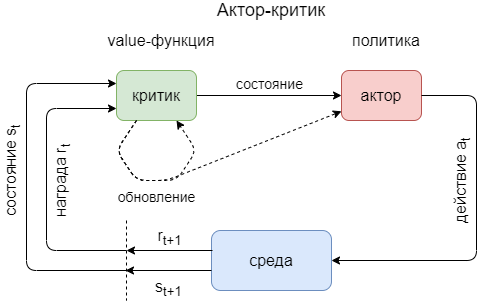
\includegraphics [scale=0.60] {my_folder/images/ch1/RL-actor-critic.png}
    \caption{Актор получает состояние из окружающей среды и реагирует на действие, критик получает состояние и награду и рассчитывает TD ошибку для обновления себя и актора. Основано на \cite{Arulkumaran_2017}}
    \label{fig:ch1-RL-actor-critic}
\end{figure}

\subsubsection{Глубокий детерминированный градиент политики (DDPG)}

\hyperref[acr:ddpg]{DDPG}~--- это актор-критик алгоритм, в котором нет модели и нет политики \cite{lillicrap2015continuous}. Он расширяет \hyperref[acr:dpg]{DPG} использованием глубоких нейронных сетей. Также, он использует хорошо зарекомендовавший себя приём DQN с текущей и целевой $Q$-сетями (сети критиков) и experience replay, чтобы стабилизировать обучение. И, наконец, он использует детерминированную политику (сеть акторов) вместо политики стохастического поведения.

В отличие от стохастической политики, которая определяет вероятность распределения через действия в данном состоянии, детерминированность в DDPG подразумевает, что конкретное действие аппроксимируется в данном состоянии. Соответственно конкретное состояние для следующего шага, также детерминировано.

Следовательно, вместо использования рекурсивного программирования, как в уравнении Беллмана, используется детерминированная политика ${\mu : S \leftarrow A}$ \cite{lillicrap2015continuous}

\begin{equation}
    \label{eq:ch1-ddpg-1}
    \begin{multlined}
        Q^\mu (s_t, a_t) = \mathbb{E}_{r_t, s_{t+1}~E}[r(s_t, a_t) + \gamma Q^\mu(s_{t+1}, \mu(s_{t+1})],
    \end{multlined}
\end{equation}
что очень похоже на $Q$-обучение – алгоритм с жадной политикой. Сеть критика обновляется по функции потерь

\begin{equation}
    \label{eq:ch1-ddpg-1}
    \begin{multlined}
        L(\theta^Q) = \mathbb{E}[(Q(s_t, a_t|\theta^Q) - y_t)^2],
    \end{multlined}
\end{equation}
где

\begin{equation}
    \label{eq:ch1-ddpg-3}
    \begin{multlined}
        y_t = r(s_t, a_t) + \gamma Q(s_{t+1}, \mu(s_{t+1})j\theta^Q).
    \end{multlined}
\end{equation}

Сеть актора обновляется функцией потерь

\begin{equation}
    \label{eq:ch1-ddpg-4}
    \begin{multlined}
        \nabla_{\theta \mu} J \approx \mathbb{E}[\nabla_{\theta \mu} Q(s, a \theta^Q)|_{s=s_t,a=\mu(s_t|\theta^\mu)}] = \\
        = \mathbb{E}[\nabla_a Q(s, a \theta^Q)|_{s=s_t,a=\mu(s_t) \nabla_{\theta \mu} \mu (s|\theta^\mu)|s=s_t}].
    \end{multlined}
\end{equation}

Как и в DQN, чтобы избежать расхождения, в DDPG применяется мягкое обновление (soft update) для целевых сетей критика и актора. Они обновляются только раз в указанное количество шагов.
